\documentclass[tikz,border=0pt]{standalone}
\usepackage{fontspec}
\newfontfamily\headingfont{Lato}
\newfontfamily\bodyfont{Liberation Sans}
\newfontfamily\geometryfont{Latin Modern Sans}
\newcommand{\nodehead}[1]{{\headingfont\bfseries #1}}
\usepackage{amsmath}
\usepackage{tikz}
\usetikzlibrary{arrows.meta, positioning, calc, fit, backgrounds}

\definecolor{fwSource}{RGB}{246,249,252}
\definecolor{fwControl}{RGB}{241,248,247}
\definecolor{fwLane}{RGB}{247,250,255}
\definecolor{fwEvidence}{RGB}{254,249,241}
\definecolor{fwSynthesis}{RGB}{244,250,245}
\definecolor{fwRepo}{RGB}{249,247,252}
\definecolor{fwGroup}{RGB}{250,250,248}

\begin{document}
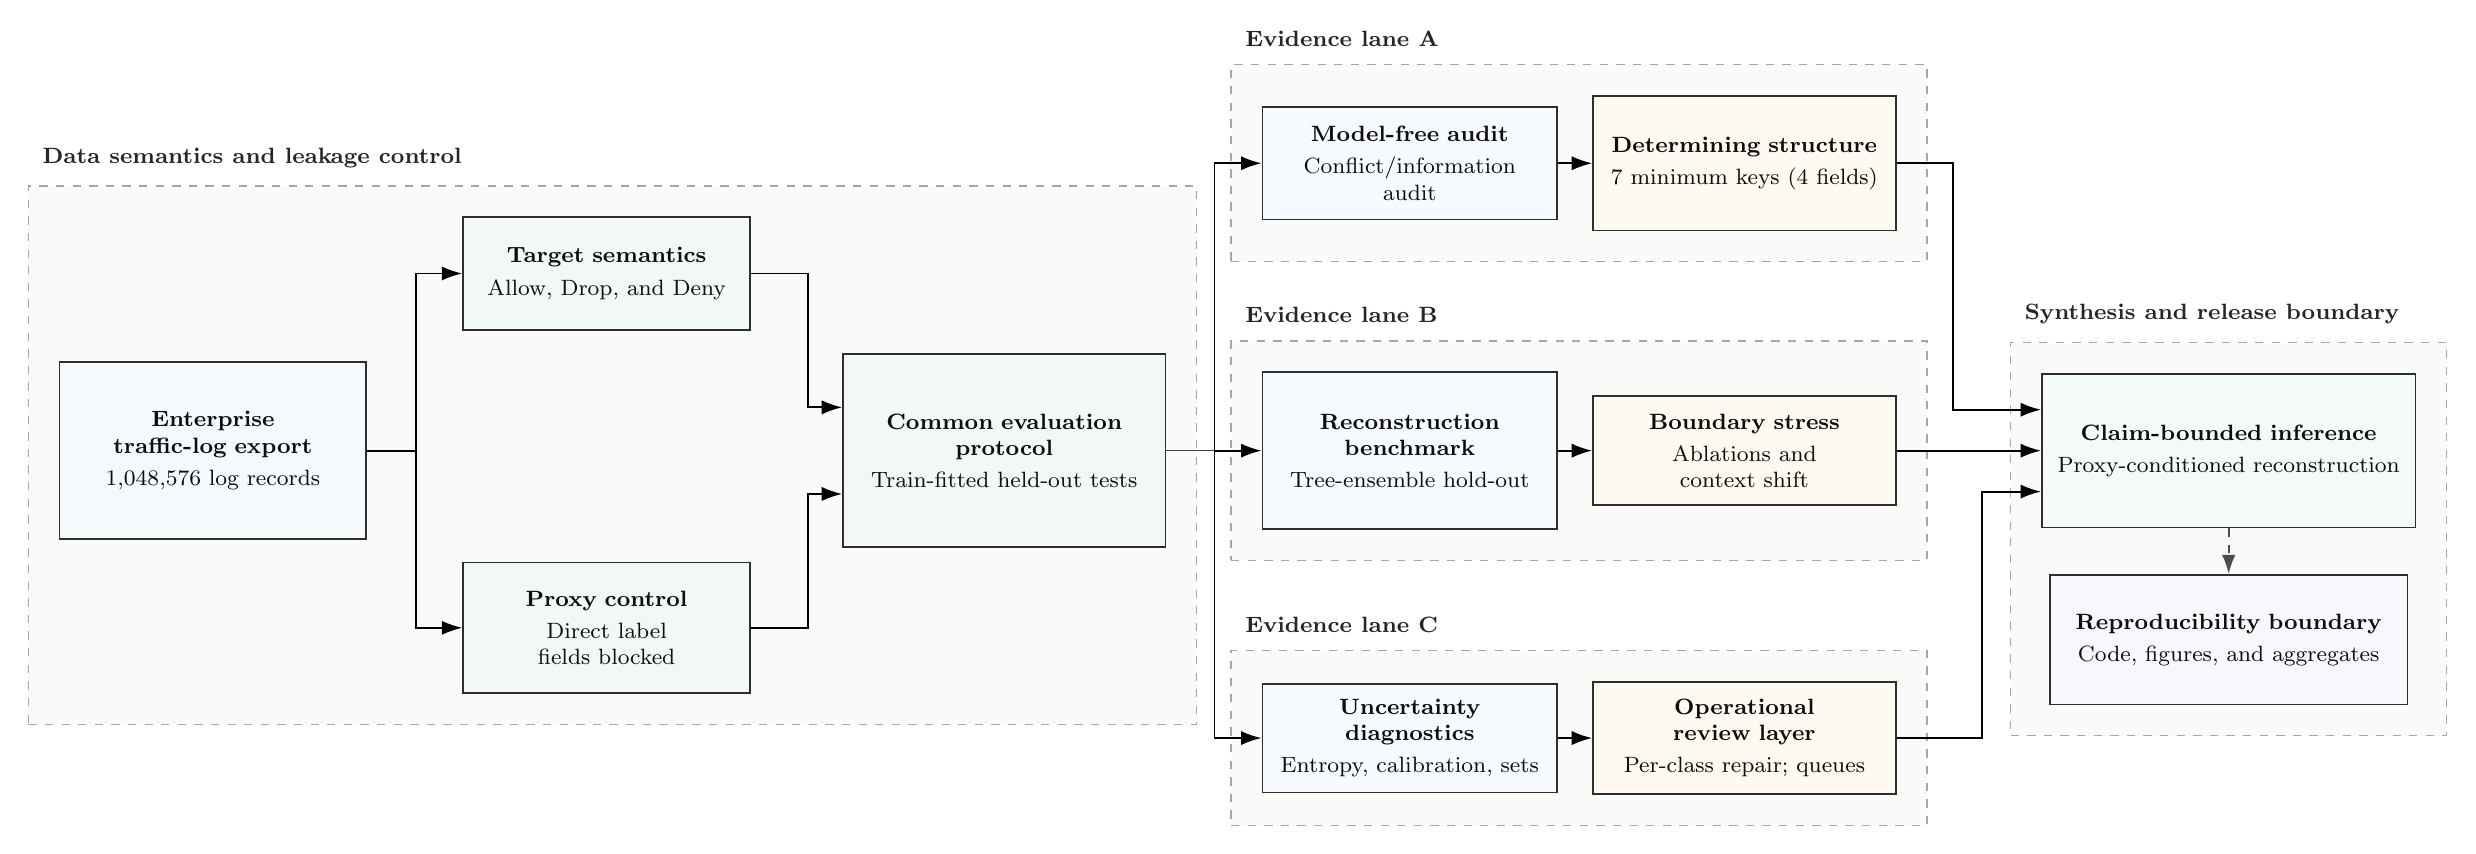
\begin{tikzpicture}[
  font=\bodyfont,
  box/.style={rectangle, draw=black!82, line width=0.60pt, fill=fwLane,
    align=center, inner sep=4.2pt, minimum height=1.22cm,
    text width=3.35cm, font=\scriptsize\geometryfont},
  source/.style={box, text width=3.60cm, minimum height=2.25cm, fill=fwSource},
  control/.style={box, fill=fwControl},
  lane/.style={box, text width=3.45cm, fill=fwLane},
  result/.style={box, text width=3.55cm, fill=fwEvidence},
  synthesis/.style={box, text width=4.45cm, minimum height=1.95cm, fill=fwSynthesis},
  repo/.style={box, text width=4.25cm, minimum height=1.65cm, fill=fwRepo},
  group/.style={rectangle, draw=black!35, line width=0.45pt, dashed,
    inner sep=11pt, fill=fwGroup},
  arr/.style={-{Latex[length=2.6mm,width=1.8mm]}, line width=0.68pt, draw=black},
  dasharr/.style={-{Latex[length=2.4mm,width=1.7mm]}, line width=0.60pt,
    draw=black!70, dashed},
  bus/.style={line width=0.60pt, draw=black!75},
  label/.style={font=\fontsize{8}{9.6}\selectfont\headingfont\bfseries,
    text=black!85, fill=white, inner sep=1.2pt},
  overlaytext/.style={font=\fontsize{8}{9.6}\selectfont\bodyfont,
    align=center, inner sep=0pt, text width=3.35cm, text=black!95}
]

% Invisible originals retain the author-approved box dimensions exactly.
\node[source, text opacity=0] (raw) at (0,0)
  {\textbf{Enterprise traffic-log export}\\[2pt]
   1{,}048{,}576 records\\ one firewall context\\ structured log fields};
\node[control, text opacity=0] (target) at (5.00,2.25)
  {\textbf{Target semantics}\\[2pt]
   Allow, Drop, Deny\\ subtype precedence\\ operational decision};
\node[control, text opacity=0] (leakage) at (5.00,-2.25)
  {\textbf{Proxy control}\\[2pt]
   direct label-source fields blocked\\ policy fields isolated\\ no attack-label claim};
\node[control, text width=3.80cm, minimum height=2.45cm, text opacity=0]
  (protocol) at (10.05,0)
  {\textbf{Common evaluation\\protocol}\\[2pt]
   train-fitted preprocessing\\ full export and capped sample\\
   random and temporal\\ held-out views};

\node[lane, text opacity=0] (auditA) at (15.20,3.65)
  {\textbf{Model-free audit}\\[2pt]
   conflict rows\\ $H(Y\mid V)$ and $\mathrm{Err}^{\star}$\\ lookup witness};
\node[result, text opacity=0] (auditB) at (19.45,3.65)
  {\textbf{Determining structure}\\[2pt]
   exhaustive census\\ of minimum keys\\ no subset with $|S|\leq3$\\ seven four-field keys};
\node[lane, text opacity=0] (benchA) at (15.20,0)
  {\textbf{Reconstruction\\benchmark}\\[2pt]
   XGBoost and LightGBM\\ full-data hold-out\\ macro-F1 and\\ balanced accuracy};
\node[result, text opacity=0] (benchB) at (19.45,0)
  {\textbf{Boundary stress}\\[2pt]
   proxy-family ablations\\ temporal split\\ context-held-out shift};
\node[lane, text opacity=0] (uncA) at (15.20,-3.65)
  {\textbf{Uncertainty diagnostics}\\[2pt]
   entropy, ECE, Brier\\ conformal prediction sets\\ calibration behavior};
\node[result, text opacity=0] (uncB) at (19.45,-3.65)
  {\textbf{Operational review layer}\\[2pt]
   Mondrian per-class repair\\ APS set expansion\\ selective-risk queues};
\node[synthesis, text opacity=0] (claim) at (25.60,0)
  {\textbf{Claim-bounded inference}\\[3pt]
   near-deterministic reconstruction\\ proxy-conditioned structure\\ residual ambiguity under shift};
\node[repo, text opacity=0] (repo) at (25.60,-2.40)
  {\textbf{Reproducibility boundary}\\[2pt]
   code, figures, aggregates\\ schema-level documentation\\ raw records withheld};

% Akis1 figure-font hierarchy: Lato Bold headings, Liberation Sans subtext.
\node[overlaytext, text width=3.60cm] at (raw.center)
  {\nodehead{Enterprise traffic-log export}\\[2pt]1{,}048{,}576 log records};
\node[overlaytext] at (target.center)
  {\nodehead{Target semantics}\\[2pt]Allow, Drop, and Deny};
\node[overlaytext] at (leakage.center)
  {\nodehead{Proxy control}\\[2pt]Direct label fields blocked};
\node[overlaytext, text width=3.80cm] at (protocol.center)
  {\nodehead{Common evaluation\\protocol}\\[2pt]Train-fitted held-out tests};
\node[overlaytext, text width=3.45cm] at (auditA.center)
  {\nodehead{Model-free audit}\\[2pt]Conflict/information audit};
\node[overlaytext, text width=3.55cm] at (auditB.center)
  {\nodehead{Determining structure}\\[2pt]7 minimum keys (4 fields)};
\node[overlaytext, text width=3.45cm] at (benchA.center)
  {\nodehead{Reconstruction\\benchmark}\\[2pt]Tree-ensemble hold-out};
\node[overlaytext, text width=3.55cm] at (benchB.center)
  {\nodehead{Boundary stress}\\[2pt]Ablations and context shift};
\node[overlaytext, text width=3.45cm] at (uncA.center)
  {\nodehead{Uncertainty diagnostics}\\[2pt]Entropy, calibration, sets};
\node[overlaytext, text width=3.55cm] at (uncB.center)
  {\nodehead{Operational review layer}\\[2pt]Per-class repair; queues};
\node[overlaytext, text width=4.45cm] at (claim.center)
  {\nodehead{Claim-bounded inference}\\[2pt]Proxy-conditioned reconstruction};
\node[overlaytext, text width=4.25cm] at (repo.center)
  {\nodehead{Reproducibility boundary}\\[2pt]Code, figures, and aggregates};

\begin{scope}[on background layer]
  \node[group, fit=(raw) (target) (leakage) (protocol)] (gdata) {};
  \node[group, fit=(auditA) (auditB)] (gaudit) {};
  \node[group, fit=(benchA) (benchB)] (gbench) {};
  \node[group, fit=(uncA) (uncB)] (gunc) {};
  \node[group, fit=(claim) (repo)] (gclaim) {};
\end{scope}

\node[label, anchor=south west] at ([xshift=4pt,yshift=5pt]gdata.north west)
  {Data semantics and leakage control};
\node[label, anchor=south west] at ([xshift=4pt,yshift=5pt]gaudit.north west)
  {Evidence lane A};
\node[label, anchor=south west] at ([xshift=4pt,yshift=5pt]gbench.north west)
  {Evidence lane B};
\node[label, anchor=south west] at ([xshift=4pt,yshift=5pt]gunc.north west)
  {Evidence lane C};
\node[label, anchor=south west] at ([xshift=4pt,yshift=5pt]gclaim.north west)
  {Synthesis and release boundary};

\draw[arr] (raw.east) -- ++(0.62,0) |- (target.west);
\draw[arr] (raw.east) -- ++(0.62,0) |- (leakage.west);
\draw[arr] (target.east) -- ++(0.72,0) |- ([yshift=0.55cm]protocol.west);
\draw[arr] (leakage.east) -- ++(0.72,0) |- ([yshift=-0.55cm]protocol.west);
\coordinate (hub) at (12.72,0);
\draw[bus] (protocol.east) -- (hub);
\draw[arr] (hub) |- (auditA.west);
\draw[arr] (hub) -- (benchA.west);
\draw[arr] (hub) |- (uncA.west);
\draw[arr] (auditA.east) -- (auditB.west);
\draw[arr] (benchA.east) -- (benchB.west);
\draw[arr] (uncA.east) -- (uncB.west);
\draw[arr] (auditB.east) -- ++(0.72,0) |- ([yshift=0.52cm]claim.west);
\draw[arr] (benchB.east) -- (claim.west);
\draw[arr] (uncB.east) -- ++(1.08,0) |- ([yshift=-0.52cm]claim.west);
\draw[dasharr] (claim.south) -- (repo.north);

\end{tikzpicture}
\end{document}
